\chapter{Testing}
In order to verify the correct behavior of our system, independent unit tests of each each subsystem were performed, before integrating them into the rest of the system. The verification of the test results was done manually and not by using a set of autonomous testbenches, as the test-driven methodology is still new and uncommon in the field of embedded systems.

\section{Unit testing}
Individual unit tests were carried out to perform a functional verification of each hardware subsystem before the different parts were put together. These unit tests were implemented in the prototyping boards and were designed to exercise the basic functionality of each sensor. The collected data was logged through the debug interfaces of the boards.

Furthermore the tests were also used to verify the current consumption of both the sensor and the MCU while executing the low energy data acquisition code. The current was logged separately and the values from the devices datasheets were verified. Energy Micro manufacturer of the EFM32GG MCU provides a tool called Energy Aware Profiler which enables the visualization and logging of tracking of real time current consumption. Using that tool some graphs were generated, two examples are included in this section for further analysis.

\begin{figure}
\centering
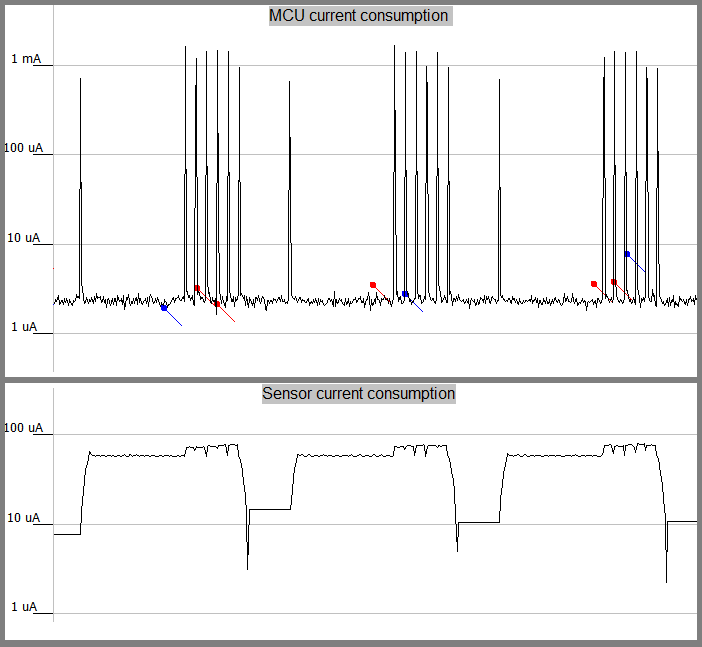
\includegraphics[width=0.6\textwidth]{Images/accel_merged}
\caption{Accelerometer power measurements}
\label{fig:accelerometer}
\end{figure}

A plot of the current consumption of the accelerometer sensor and the MCU can be seen in figure \ref{fig:accelerometer} on top and bottom graphs respectively. As can be seen on the graphs, when the accelerometer is in the sleep mode the power consumption of the sensor is around 10 uA. Then the MCU wakes up the accelerometer (single peak) and the accelerometer collects 5 samples, during this period current consumption of the sensor is around 60 uA. After the sample collection, the accelerometer sends the data to the MCU and in this phase the current consumption is at its highest level for both which is approximately 70 uA for the accelerometer.


\begin{figure}
\centering
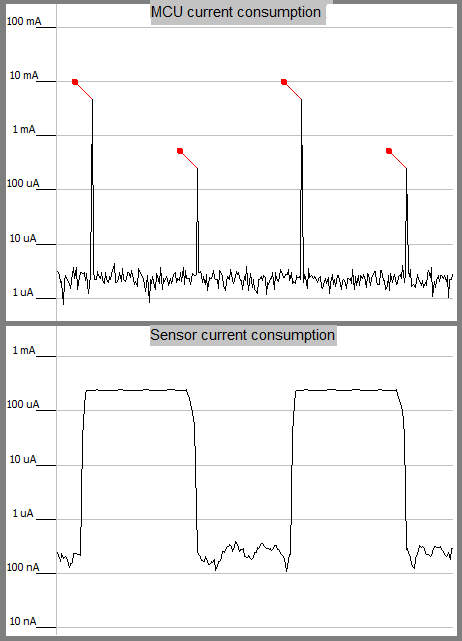
\includegraphics[width=0.6\textwidth]{Images/tmp_merged}
\caption{Temperature sensor power measurements}
\label{fig:temp_sensor}
\end{figure}

The power profile for the temperature subsystem can be seen in the figure \ref{fig:temp_sensor}. In this case the current drawned by the temperature sensor is of 241 uA while active and it goes down to 38 uA when the device enters sleep mode. As we can see in the top graph the cpu sleeps most of the time and only wakes up shortly twice per sample collection. While sleeping the current consumption of the MCU is between 2 and 3 uA which is compatible with the datasheet.


\section{Wireless communication}
\label{sec:wireless_testing}
The functionality of our system depends on a wireless connection, which is why we needed to ensure that we can guarantee a stable connection and reliable transmission of data over the wireless link, while being able to transmit data at a reasonable data rate.

To verify that the connection fulfils these requirements we ran a stress test, where two devices, one configured as network coordinator, the other configured as a network node, exchanged small data packets over a long period of time (>4h). 

The reliability of the transmitted data was tested by sending a predictable set of values between the network nodes and aborting the test when receiving a value that differs from the expected value. 

The stability of the connection was tested by imposing a timeout limit on both sides of the connection. If no data was received within a defined timeframe or no acknowledgement was received the test was also aborted.

When the system passed this stress test and we could rely on a stable and reliable connection we had to verify the last of the three requirements - the data throughput.

To test the data throughput we used the XBee interface we had developed to transmit messages larger than the maximal ZigBee frame size. The throughput was obtained by sending a defined amount of data and measuring the delay between sending and receiving the acknowledgment for the last part of the message. The results can be seen in figure \ref{fig:xbee_throughput}.

\begin{figure}
\centering
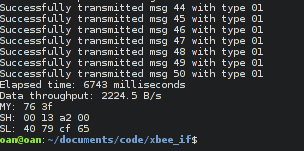
\includegraphics[width=0.5\textwidth]{Images/xbee_throughput}
\caption{XBee throughput}
\label{fig:xbee_throughput}
\end{figure}

The throughput test revealed that the chosen wireless protocol is not able to transmit data nearly as fast as we expected. The maximal throughput that can be reached by our system is 13kbits/s, which is about 20 times slower than what we had expected (ZigBee data rate is often quoted as  250kbit/s). 

It turned out that the firmware for the devices we are using (XBee) imposes a large additional overhead on the protocol and that even using a pure ZigBee implementation the data rate of 250kbit/s can never be reached, because the ZigBee standard itself uses part of the data rate to implement its functionality and vendor specific ZigBee implementations add even more overhead. The XBee device manual states this in a subsection, that we didn’t take into account during the design phase. The maximal data rate that is specified for network using our configuration is 16kbit/s.

This result has a strong influence on our system, because it renders wireless transmission of audio data infeasible. A small calculation shows why

\begin{flalign}
t_{transmission} &= \frac{data rate*t_{duration}}{f_{transmission}} \\
& = \frac{128kbit/s*240s}{13kbit/s} \\
& = 39min
\end{flalign}

It takes 39 minutes to transmit a 4 minute gut sound recording, which conflicts with our goal of a battery powered energy efficient system, because the processor has to be awake while transmitting the data over ZigBee and the battery runtime would decrease drastically.

The current solution for this problem, is to store audio recording on a removable SD card in the monitoring device. Proper solutions for this problem are discussed in the Future Work Chapter (\ref{sec:future_work})

\section{System Integration testing}
\begin{figure}
\centering
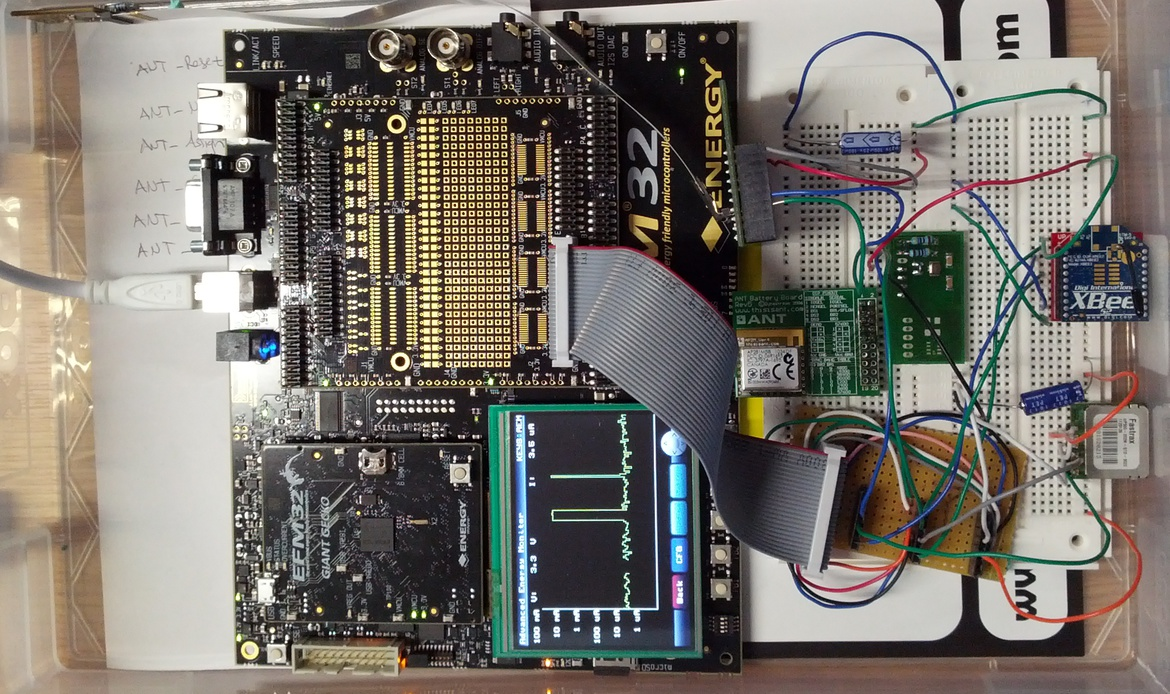
\includegraphics[width=0.9\textwidth]{Images/integration_crop}
\caption{System Integration on Energy Micro DK}
\label{fig:integration}
\end{figure}
After the individual hardware subsystem prototypes had been verified, the units were connected to build a prototype of the complete system. Gradually all the sensors were integrated to the final monitoring device PCB prototype. Integration testing was done on the Energy Micro DK and integrated software debugging was done before the PCB was received. The prototype can be seen in figure \ref{fig:integration}.

In this stage, the monitoring device with its subsystems and the base station were tested. Measurement data was successfully transferred from the monitoring device over the wireless link and stored in the database in the base station. After the prototype of the complete system was tested and verified the modules were soldered on the PCB.

The final stage of integration on the PCB went without problems, or required changes to the software of the system.  



\section{Field Testing}
Throughout the development process, the team did not have access to a horse and there is almost no sample gut sound recordings available online. After the integration and PCB production phases were complete, the system was tested on human subjects since the subsystems of the monitoring device are usable on humans as well. The only horse-specific part of the system was the gut sound monitor - although it is also usable on humans, the design was not made with humans or species other than horses in mind. 

In the laboratory environment, the team could only test the gut sound monitor on human subjects to record heart beats since human gut sounds are not as periodic and loud as those of a horse. Human heart beat recordings were made without problems, and four beats of an approximately 65 BPM heartbeat with the S\_1 and S\_2 (respectively the "lub" and "dub" sounds) can be clearly seen in figure \ref{fig:heartbeat}

\begin{figure}
\centering
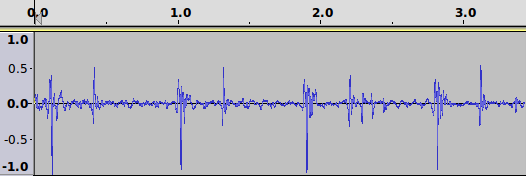
\includegraphics[width=0.8\textwidth]{Images/heartbeat.png}
\caption{Testing results: heartbeat}
\label{fig:heartbeat}
\end{figure}

However, this is not the real usage of the module. Thus, the team made a field trip to New Forest to perform gut sound monitor testing on equines. Gut sounds of three horses were recorded from different sites of the abdomen. Each recording was done one minute long and saved in the SD card. The result was satisfactory although the environment was noisy because of the horses' movements and conversations. Therefore, noise cancellation filter is needed to improve the performance. The recordings can be found in the Appendix \ref{sec:gut_sound_recordings}.

\begin{itemize}
\item no gut sound recording was available on web
\item we could test the integrated system (temperature etc on humans) but gut sound is horse-specific so we arranged a field trip. (TODO{} not sure if we should add thıs ınfo: + testing the whole components on gut requires more time, components and people) and it was not crucial, because complete system testing was successful.
\item we did gut sound recording on 3 horses from different parts of the abdomen, each 1 minute long. although the environment was noisy (horse was moving, conversations etc) the recordings were successful. They can be found in appendix. A noise filtering needed to get better results.
\end{itemize}


